\documentclass[
 size=14pt,
 paper=smartboard,  % a4paper, smartboard, screen
 mode=present, 		% present, handout, print
 display=slides, 	% slidesnotes, notes, slides
 style=tuliplab,  	% TULIP Lab style
 pauseslide,
 fleqn,leqno]{powerdot}{}

 %=================================================================
%
% ---------------------------------------------------------------
% Copyright (C) 2012-2018 Gang Li
% ---------------------------------------------------------------
%
% This work is the default powerdot-tuliplab style test file and may be
% distributed and/or modified under the conditions of the LaTeX Project Public
% License, either version 1.3 of this license or (at your option) any later
% version. The latest version of this license is in
% http://www.latex-project.org/lppl.txt and version 1.3 or later is part of all
% distributions of LaTeX version 2003/12/01 or later.
%
% This work has the LPPL maintenance status "maintained".
%
% This Current Maintainer of this work is Gang Li.
%
%
\usepackage{smartdiagram}
\usepackage{amssymb}
\usepackage{amsmath}
\usepackage{rotating}
\usepackage{graphicx}
\usepackage{boxedminipage}
\usepackage{media9}
\usepackage{rotate}
\usepackage{calc}
\usepackage[absolute]{textpos}
\usepackage{psfrag,overpic}
\usepackage{fouriernc}
\usepackage{pstricks,pst-node,pst-text,pst-3d,pst-grad}
\usepackage{moreverb,epsfig,subfigure}
\usepackage{pstricks}
\usepackage{pstricks-add}
\usepackage{pst-text}
\usepackage{pst-node, pst-tree}
\usepackage{booktabs}
\usepackage{etex}
\usepackage{breqn}
\usepackage{multirow}
\usepackage{gitinfo2}
\usepackage{xcolor}
\usepackage{multicol}
\usepackage{ulem}
\usepackage{todonotes}
\usepackage{tablefootnote}
\usepackage{threeparttable}
\usepackage[numbers]{natbib}
\usepackage{bibentry}
% \usepackage{pst-rel-points}
\usepackage{pgfplots}
\usepackage{verbatim}
\usepackage{fontawesome}
\usepackage{multirow}
\usepackage{tikz}
\usetikzlibrary{shapes,snakes}
\usetikzlibrary{shapes.symbols,positioning}
\usepackage{amsmath,amssymb}



%\usepackage{graphicx}
\usepackage{animate}

\usepackage{listings}
\lstset{frameround=fttt,
frame=trBL,
stringstyle=\ttfamily,
backgroundcolor=\color{yellow!20},
basicstyle=\footnotesize\ttfamily}
\lstnewenvironment{code}{
\lstset{frame=single,escapeinside=`',
backgroundcolor=\color{yellow!20},
basicstyle=\footnotesize\ttfamily}
}{}


\usepackage{hyperref}
\hypersetup{ % TODO: PDF meta Data
  pdftitle={TULIP Lab},
  pdfauthor={Gang Li},
  pdfpagemode={FullScreen},
  pdfborder={0 0 0}
}



% \usepackage{auto-pst-pdf}
% package to show source code

%\definecolor{LightGray}{rgb}{0.9,0.9,0.9}
\definecolor{antiquebrass}{rgb}{0.8, 0.58, 0.46}
\newlength{\pixel}\setlength\pixel{0.000714285714\slidewidth}
\setlength{\TPHorizModule}{\slidewidth}
\setlength{\TPVertModule}{\slideheight}
\newcommand\highlight[1]{\fbox{#1}}
\newcommand\icite[1]{{\footnotesize [#1]}}

\newcommand\twotonebox[2]{\fcolorbox{pdcolor2}{pdcolor2}
{#1\vphantom{#2}}\fcolorbox{pdcolor2}{white}{#2\vphantom{#1}}}
\newcommand\twotoneboxo[2]{\fcolorbox{pdcolor2}{pdcolor2}
{#1}\fcolorbox{pdcolor2}{white}{#2}}
\newcommand\vpspace[1]{\vphantom{\vspace{#1}}}
\newcommand\hpspace[1]{\hphantom{\hspace{#1}}}
\newcommand\COMMENT[1]{}

\newcommand\placepos[3]{\hbox to\z@{\kern#1
        \raisebox{-#2}[\z@][\z@]{#3}\hss}\ignorespaces}

\renewcommand{\baselinestretch}{1.2}


\newcommand{\draftnote}[3]{
	\todo[author=#2,color=#1!30,size=\footnotesize]{\textsf{#3}}}
% TODO: add yourself here:
%
\newcommand{\gangli}[1]{\draftnote{blue}{GLi:}{#1}}
\newcommand{\shaoni}[1]{\draftnote{green}{sn:}{#1}}
\newcommand{\mengren}[1]{\draftnote{orange}{MRen:}{#1}}
\newcommand{\xinhan}[1]{\draftnote{red}{Xhan:}{#1}}
\newcommand{\gliMarker}
	{\todo[author=GLi,size=\tiny,inline,color=blue!40]
	{Gang Li has worked up to here.}}
\newcommand{\snMarker}
	{\todo[author=Sn,size=\tiny,inline,color=green!40]
	{Shaoni has worked up to here.}}
\newcommand{\mrMarker}
	{\todo[author=MRen,size=\tiny,inline,color=orange!40]
	{Meng Ren has worked up to here.}}
\newcommand{\xhMarker}
	{\todo[author=XHan,size=\tiny,inline,color=red!40]
	{XinHan has worked up to here.}}
\newcommand{\zhMarker}
{\todo[author=ZHou,size=\tiny,inline,color=purple!40]
	{Ziwei Hou has worked up to here.}}

\usepackage{geometry}
\geometry{verbose,letterpaper}
\usepackage{movie15}
\usepackage{hyperref}

\usepackage[utf8]{inputenc}
\usepackage{dtk-logos}
\usepackage{tikz}
\usetikzlibrary{arrows,chains,mindmap,shadows,automata,patterns,
	petri,shapes.geometric,shapes.misc, spy, trees,decorations.markings}
%\usepackage[hidelinks,pdfencoding=auto]{hyperref}
% Information boxes
\newcommand*{\info}[4][4]{%
  \node [ annotation, #3, text width = 3.35cm,
          inner sep = 0.3em ] at (#2) {%
  \list{$\bullet$}{\topsep=-3pt\itemsep=0pt\parsep=1pt
    \parskip=1pt\labelwidth=0pt\leftmargin=1pt
    \itemindent=1pt\labelsep=1pt}%
    #4
  \endlist
  };
}

\newcommand*{\infoo}[4][4]{%
  \node [ annotation, #3, text width = 2.7cm,
          inner sep = 0.3em ] at (#2) {%
  \list{$\bullet$}{\topsep=-3pt\itemsep=0pt\parsep=1pt
    \parskip=1pt\labelwidth=0pt\leftmargin=1pt
    \itemindent=1pt\labelsep=1pt}%
    #4
  \endlist
  };
}

% aiming high
\usepackage{smartdiagram}
\usetikzlibrary{shapes.symbols}


\tikzstyle{mybox} = [draw=red, fill=blue!20, very thick,
    rectangle, rounded corners, inner sep=10pt, inner ysep=20pt]
\tikzstyle{fancytitle} =[fill=red, text=white]


\tikzset{description title/.append style={
%    signal,
%    signal to=south,
%    signal from=nouth,
    yshift=0.1cm,
  }
}


%forest
\usepackage{forest}
\usetikzlibrary{arrows.meta, shapes.geometric, calc, shadows}

\colorlet{mygreen}{green!75!black}
\colorlet{col1in}{red!30}
\colorlet{col1out}{red!40}
\colorlet{col2in}{mygreen!40}
\colorlet{col2out}{mygreen!50}
\colorlet{col3in}{blue!30}
\colorlet{col3out}{blue!40}
\colorlet{col4in}{mygreen!20}
\colorlet{col4out}{mygreen!30}
\colorlet{col5in}{blue!10}
\colorlet{col5out}{blue!20}
\colorlet{col6in}{blue!20}
\colorlet{col6out}{blue!30}
\colorlet{col7out}{orange}
\colorlet{col7in}{orange!50}
\colorlet{col8out}{orange!40}
\colorlet{col8in}{orange!20}
\colorlet{linecol}{blue!60}

\definecolor{mynodecolor}{RGB}{198,191,234}


\pgfkeys{/smart diagram/.cd,
additions/.style={/smart diagram/additions/.cd,#1}%
}



%=================================================================
%

%%%%%%%%%%%%%%%%%%%%%%%%%%%%%%%%%%%%%%%%%%%%%%%%%%%%%%%%%%%%%%%%%%%%%%%%
% title
% TODO: Customize to your Own Title, Name, Address
%
\title{Research Material Management and Critical Thinking}
\author{
Meng Ren
\\
\\School of Computer Science and Technology
\\Xi'an Shiyou University, China
}
\date{\gitCommitterDate}


% Customize the setting of slides
\pdsetup{
% TODO: Customize tlhe left footer, and right footer
rf=\href{http://www.tulip.org.au}{
Last Changed by: \textsc{\gitCommitterName}\ \gitVtagn-\gitAbbrevHash\ (\gitAuthorDate)
},
cf={TULIP Academy},
}

\begin{document}

\maketitle

%%==========================================================================================
%%
\begin{slide}[toc=,bm=]{Overview}
\tableofcontents[content=currentsection,type=1]
\end{slide}
%%
%%==========================================================================================

%%==========================================================================================
%%
\begin{slide}[toc=,bm=]{Management, Analysis and Critical Thinking}
\begin{center}
\selectcolormodel{rgb}

\smartdiagramset{description title text width=1.5cm,
    description text width=7cm,description width=10cm}

\smartdiagram[descriptive diagram]{
  {First,Research Materials Management}}
\smartdiagram[descriptive diagram]{
  {Second,Research Summary and Analysis}}
\smartdiagram[descriptive diagram]{
  {Third,Critical Thinking}}
\end{center}

%\begin{itemize}
%  \item Management
%  \item Research Summary and Analysis
%  \begin{itemize}
%  \item Research Analysis
%  \item Research Summary
%  \end{itemize}
%  \item Critical Thinking
%\end{itemize}


\end{slide}
%%==========================================================================================

\section{Research Materials Management}

\begin{slide}{Information Acquisition}

There are too many way to find paper: \texttt{CCF}, \texttt{Google Scholar}, \texttt{arXiv} and etc.\\
There provide a way to search and collect the paper:
\begin{itemize}
  \item Search in \url{http://www.ccf.org.cn/xspj/gyml/}
  \item Choose the relevant category.
  \item Choose the relevant Journal.
  \item Choose the paper and get DOI.
  \item Download the paper from Sci-hub(\url{http://www.sci-hub.tw/})
\end{itemize}


\end{slide}
%%
%%==========================================================================================

%%==========================================================================================
%%
\begin{slide}[toc=,bm=]{Information Acquisition}

In general, we can acquire the information for \texttt{Blog}, \texttt{WeChat}, \texttt{ZhiHu,Quora},
\texttt{Feedly}, \texttt{Reddit},\texttt{Twitter} and etc.

%\begin{center}%
\begin{figure}
  \centering
  % Requires \usepackage{graphicx}
  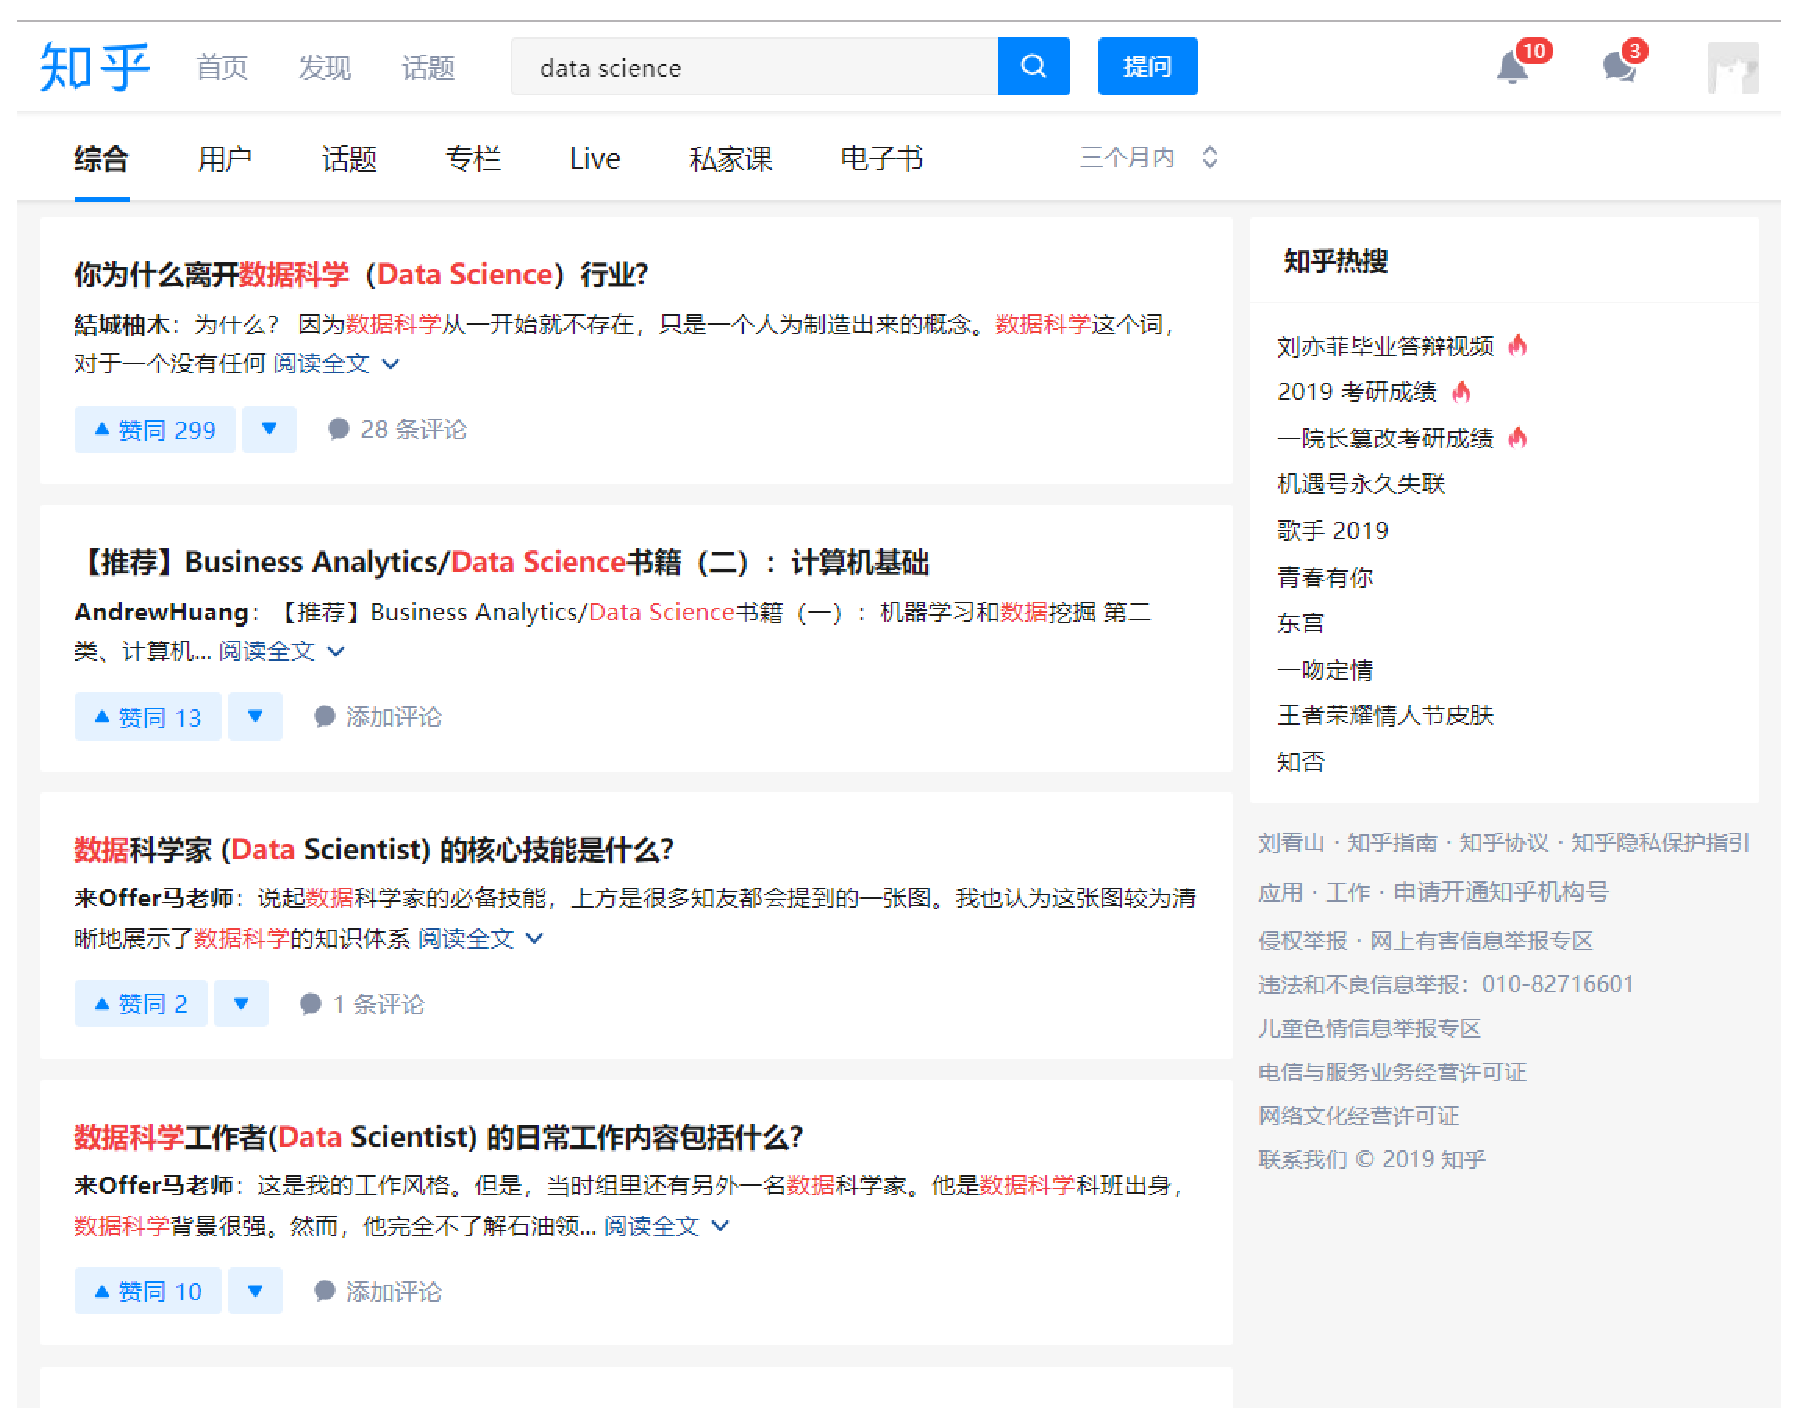
\includegraphics[width=3.2in]{figures/management/zhihu.eps}\\
%  \caption{Android}
\end{figure}
%\end{center}

\begin{itemize}
  \item Web and mobile (Vision).
  \item Browse for content of interest.
  \item Ask question.
\end{itemize}

\end{slide}
%%
%%==========================================================================================

%%==========================================================================================
%%
\begin{slide}{PDF Management}

\begin{figure}
  \centering
  % Requires \usepackage{graphicx}
  
\includegraphics[width=0.8in]{figures/management/Mendeley_Logo.eps}\\
%  \caption{Mendeley_Logo}
\end{figure}

Mendeley:

\begin{itemize}
  \item A desktop and web program.
  \item Managing and sharing research papers, discovering research data and collaborating online.
  \item Combines Mendeley Desktop, a PDF and reference management application available for Windows, macOS and Linux.
  \item Provides Mendeley for Android and iOS, with Mendeley Web, an online social network for researchers.
\end{itemize}

\textcolor{orange}{\href{https://www.zotero.org/}{\texttt{Zotero}}} is another free and open-source reference management software to manage bibliographic data and related research materials (such as PDF files).

\end{slide}
%%
%%==========================================================================================

%%==========================================================================================
%%
\begin{slide}[toc=,bm=]{PDF Management}

\twocolumn[lcolwidth=0.5\linewidth,
rcolwidth=0.5\linewidth
]{
\onslide*{1,1-}{
\begin{figure}
  \centering
  % Requires \usepackage{graphicx}
  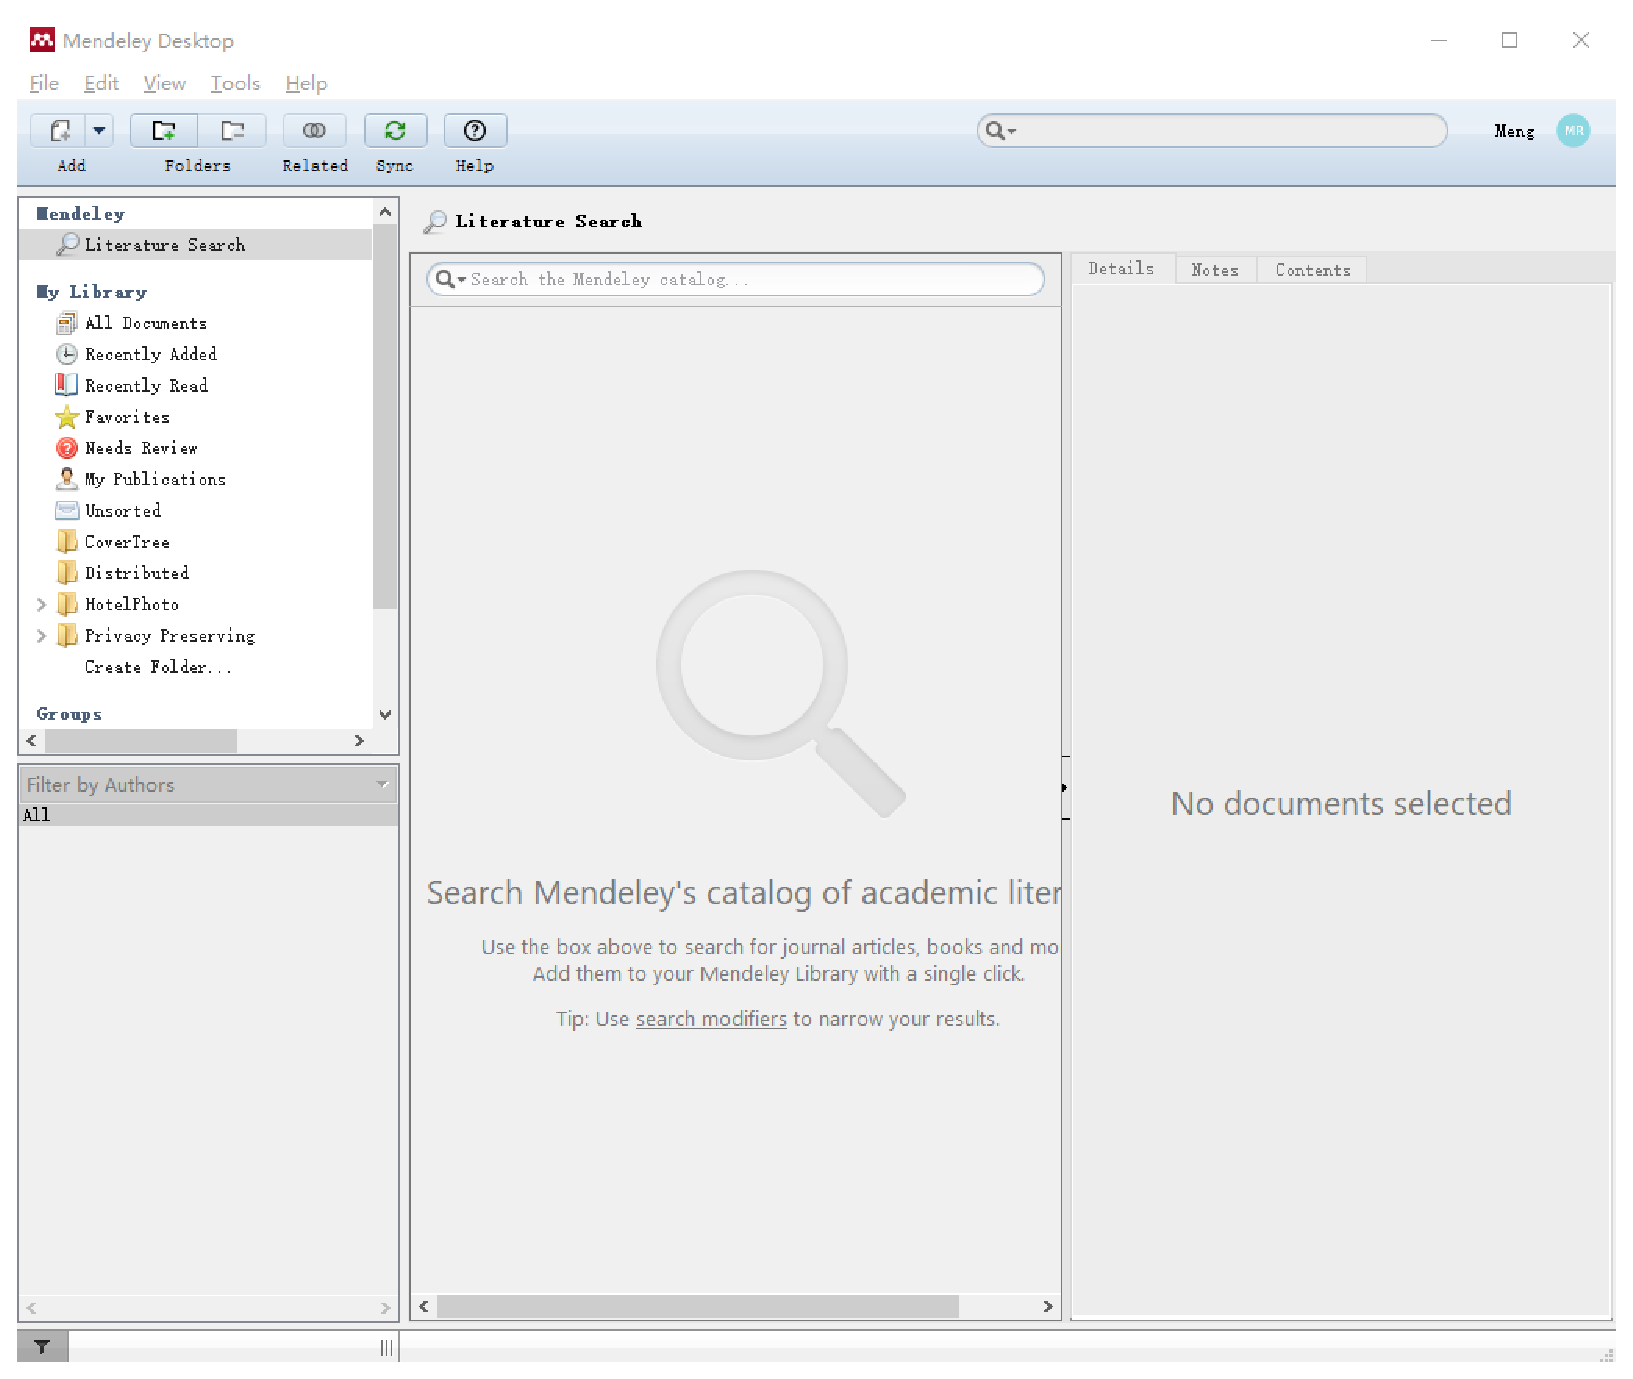
\includegraphics[width=4in]{figures/management/windows.eps}\\
  \caption{Windows}
\end{figure}}
}
{\onslide*{2,2-}{
\begin{figure}
  \centering
  % Requires \usepackage{graphicx}
  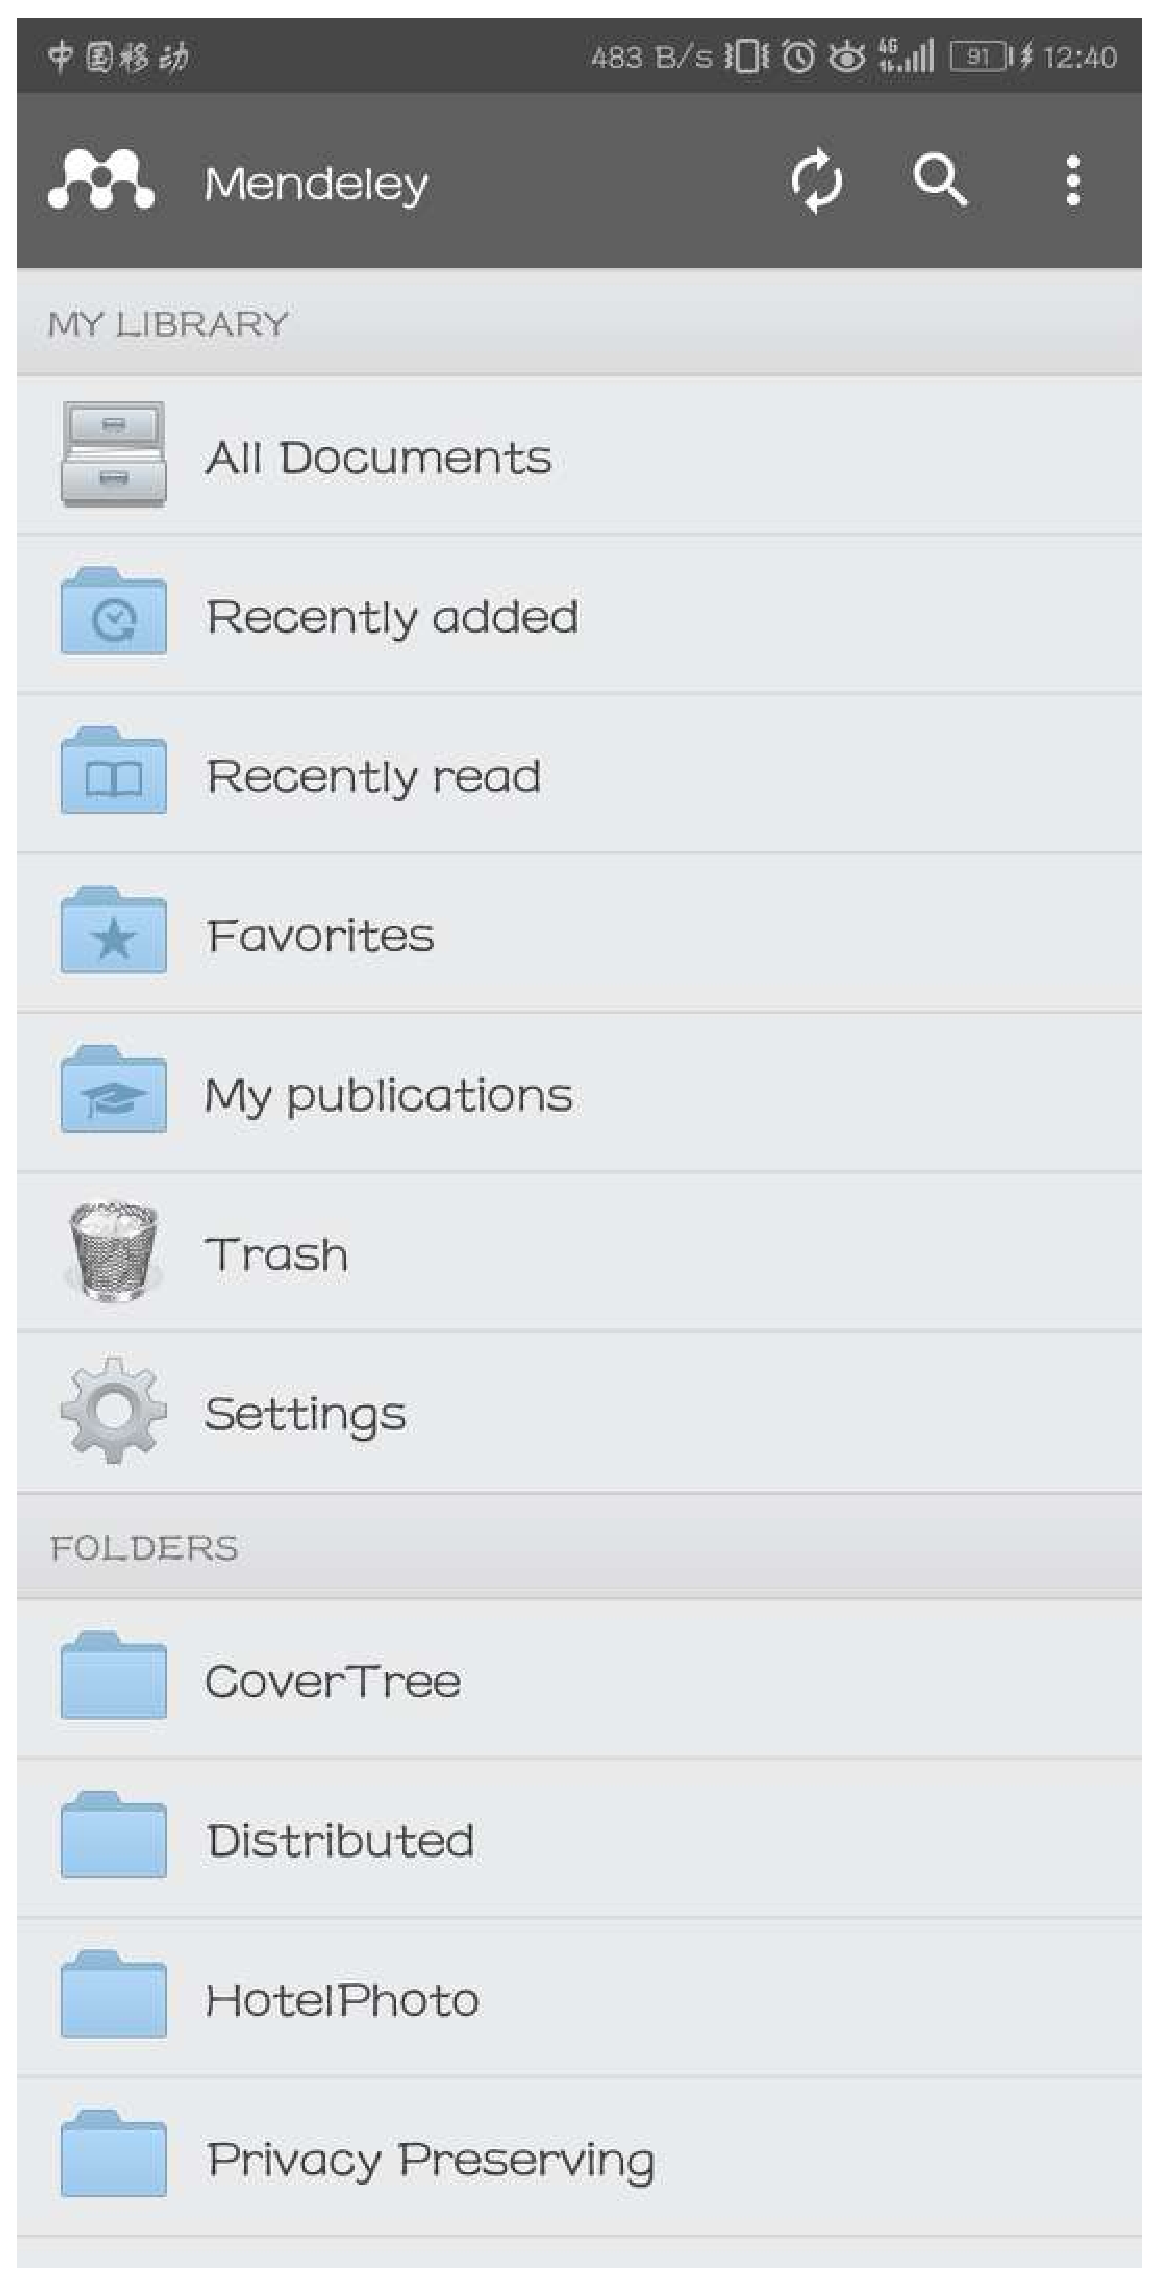
\includegraphics[width=1.5in]{figures/management/andro.eps}\\
  \caption{Android}
\end{figure}}
}
%\href{link}{https://blog.tulip.org.au/2018/04/21/Tools-Info-Management/}%
\end{slide}
%%
%%==========================================================================================


%%==========================================================================================
%%
\begin{slide}{Information Management}

\begin{figure}
  \centering
  % Requires \usepackage{graphicx}
  
\includegraphics[width=2.6in]{figures/management/computer.eps}\\
%  \caption{Mendeley_Logo}
\end{figure}

\onslide*{2,2-}{
\begin{center}
\large{\texttt{System Breakdown, Computer Damage, Lose the Document and etc.}}
\end{center}
}

\onslide*{3}{In order to avoid the above problem,
we choose Cross-Platform software in different Operating System,
such as:
\begin{center}
\textcolor{orange}{\texttt{Windows, OS X, Linux}}
\end{center}
}

\onslide*{4,4-}{
\begin{itemize}
  \item \textcolor{orange}{\textit{Baidu Drive}}: 2T free space, a Cloud service provided by \textit{Baidu}.
      %It offers a cloud storage service, client software, file management, resources sharing, and Third Party Integration.
  \item \textcolor{orange}{\textit{OneDrive}}: 10G free space for PPTX and OneNote.
  \item \textcolor{orange}{\textit{GoogleDrive}}: 15G free space for Google edit document online. (VPN)
  \item \textcolor{orange}{\textit{Bitbucket}}: Collaborative version control (Article writing).
  \item \textcolor{orange}{\textit{Github}}: a web-based hosting service for version control using Git.
\end{itemize}
}

\end{slide}
%%
%%==========================================================================================

%%==========================================================================================
%%
\begin{slide}{System backup}

Try to use cross-platform software:

\twocolumn[lcolwidth=0.5\linewidth,
rcolwidth=0.5\linewidth
]{
\onslide*{1,1-}{
\begin{figure}
  \centering
  % Requires \usepackage{graphicx}
  
\includegraphics[width=2.3in]{figures/management/office.eps}\\
  %\caption{Windows}
\end{figure}

\begin{itemize}
  \item Microsoft Word: a word processor.
  \item Microsoft Excel: a spreadsheet editor.
  \item Microsoft PowerPoint: a presentation program.
  \item Microsoft Access: a database management system.
  \item \textcolor{orange}{Microsoft OneNote}: a notetaking program.
%  \item Microsoft Publisher:  a desktop publishing app.
  \item ...
\end{itemize}

}}
{
{\onslide*{2,2-}{
\begin{figure}
  \centering
  % Requires \usepackage{graphicx}
  
\includegraphics[width=2in]{figures/management/smartgit.eps}\\
  %\caption{Android}
\end{figure}

\begin{itemize}
  \item SmartGit is a graphical client program
  for the \textcolor{orange}{\texttt{Git version control system}}.
  It has the functions of quickly establishing branches,
  supporting offline submission to the server,
  and intuitive local update,
  \textcolor{orange}{\texttt{submission}, \texttt{merge}, \texttt{refresh}},
  and \textcolor{orange}{\texttt{synchronization operations}}.
\end{itemize}
}
}}


\end{slide}
%%
%%==========================================================================================

\section{Research Summary and Analysis}

%%==========================================================================================
%%
\begin{slide}[toc=,bm=]{Research Summary and Analysis}

\begin{itemize}
  \item Paper can be divided into Two class:
  \begin{itemize}
    \item  \textcolor{orange}{\textit{Research}}: In response to new questions, propose new original theories, new evidence or new solutions (often a small research sub-question, just read the literature related to the research sub-question)
    \item  \textcolor{orange}{\textit{Survey}}: A retrospective paper that presents a variety of existing research findings and current status within the scope of a research topic. (Generally top or senior scholars.)
  \end{itemize}
\end{itemize}
\end{slide}
%%
%%==========================================================================================

%%==========================================================================================
%%
\begin{slide}{Analysis}

\begin{itemize}
    \item Method of reading papers
    \begin{itemize}
      \item Take a cursory look at it and study \textcolor{orange}{the background knowledge} that you lack, and belong to the academic branch. And find relevant literature to read.
      \item Pick out \textcolor{orange}{related chapters, pages, paragraphs} to read, and skip irrelevant content.
      \item After the background knowledge is added, look at the article that you need to read.
      \begin{itemize}
        \item Abstract
        \item Introduction
        \item Experiment
        \item Method
      \end{itemize}
    \end{itemize}
\end{itemize}
\end{slide}
%%
%%==========================================================================================

%%==========================================================================================
%%
\begin{slide}{Summary}

\begin{figure}
  \centering
  % Requires \usepackage{graphicx}
  
\includegraphics[width=3in]{figures/management/Summary.eps}\\
%  \caption{Mendeley_Logo}
\end{figure}

\begin{itemize}
  \item Summary
  \begin{itemize}
    \item \textcolor{orange}{\textit{Survey}}

    \item \textcolor{orange}{\textit{Blog}}: \href{Blog}{https://mren.tulip.academy}

    \item \textcolor{orange}{\textit{Idea Bank}}: Reading Notes

  \end{itemize}
\end{itemize}

\vspace{0.5cm}
\begin{center}
\Large{\textit{We need to develop good daily routines and record habits!}}
\end{center}
\end{slide}
%%
%%==========================================================================================

%%==========================================================================================
%%
\begin{slide}[toc=,bm=]{Summary}

\begin{figure}
  \centering
  % Requires \usepackage{graphicx}
  
\includegraphics[width=3in]{figures/management/survey.eps}\\
%  \caption{Mendeley_Logo}
\end{figure}

  \begin{itemize}
    \item \textcolor{orange}{\textit{Research Survey}}
         \begin{itemize}
           \item A Survey is defined as a research method used for collecting data from a pre-defined group of respondents to \textcolor{orange}{gain information} and insights on \textcolor{orange}{various topics of interest}. Surveys have a variety of purposes and can be carried out in many ways depending on the \textcolor{orange}{methodology chosen} and the \textcolor{orange}{objectives} to be achieved.
           \item It is often a long process to write a review of research papers. Literature review is often used to answer questions and doubts that you have raised, so that you can learn better.
         \end{itemize}
  \end{itemize}
\end{slide}
%%
%%==========================================================================================

%%==========================================================================================
%%
\begin{slide}[toc=,bm=]{Summary}

\twocolumn[lcolwidth=0.5\linewidth,
rcolwidth=0.5\linewidth
]{
\onslide*{1,1-}{
\begin{figure}
  \centering
  % Requires \usepackage{graphicx}
  
\includegraphics[width=1in]{figures/management/Blog.eps}\\
  %\caption{Windows}
\end{figure}

\begin{itemize}
    \item \textcolor{orange}{\textit{Blog}}
       \begin{itemize}
         \item When we have a new understanding of a small research topic, try to record it and give it. Thus, the more you write, the more you summarize the more you gain.
       \end{itemize}
  \end{itemize}
}}
{
{\onslide*{2,2-}{
\begin{figure}
  \centering
  % Requires \usepackage{graphicx}
  
\includegraphics[width=1.5in]{figures/management/IdeaBank.eps}\\
  %\caption{Android}
\end{figure}

\begin{itemize}
    \item \textcolor{orange}{\textit{Idea Bank}}
      \begin{itemize}
        \item At any chance when read papers,there can be a new idea, but it can't be completed immediately, you need to collect the idea. When there is no problem to do, you can go to the content collected before.
      \end{itemize}
  \end{itemize}
}
}}
\end{slide}
%%
%%==========================================================================================

\section{Critical Thinking}

%%==========================================================================================
%%
\begin{slide}[toc=,bm=]{Critical Thinking}

\begin{itemize}
  \item Critical thinking is the objective analysis of facts to form a judgment.
\end{itemize}

\begin{figure}
  \centering
  % Requires \usepackage{graphicx}
  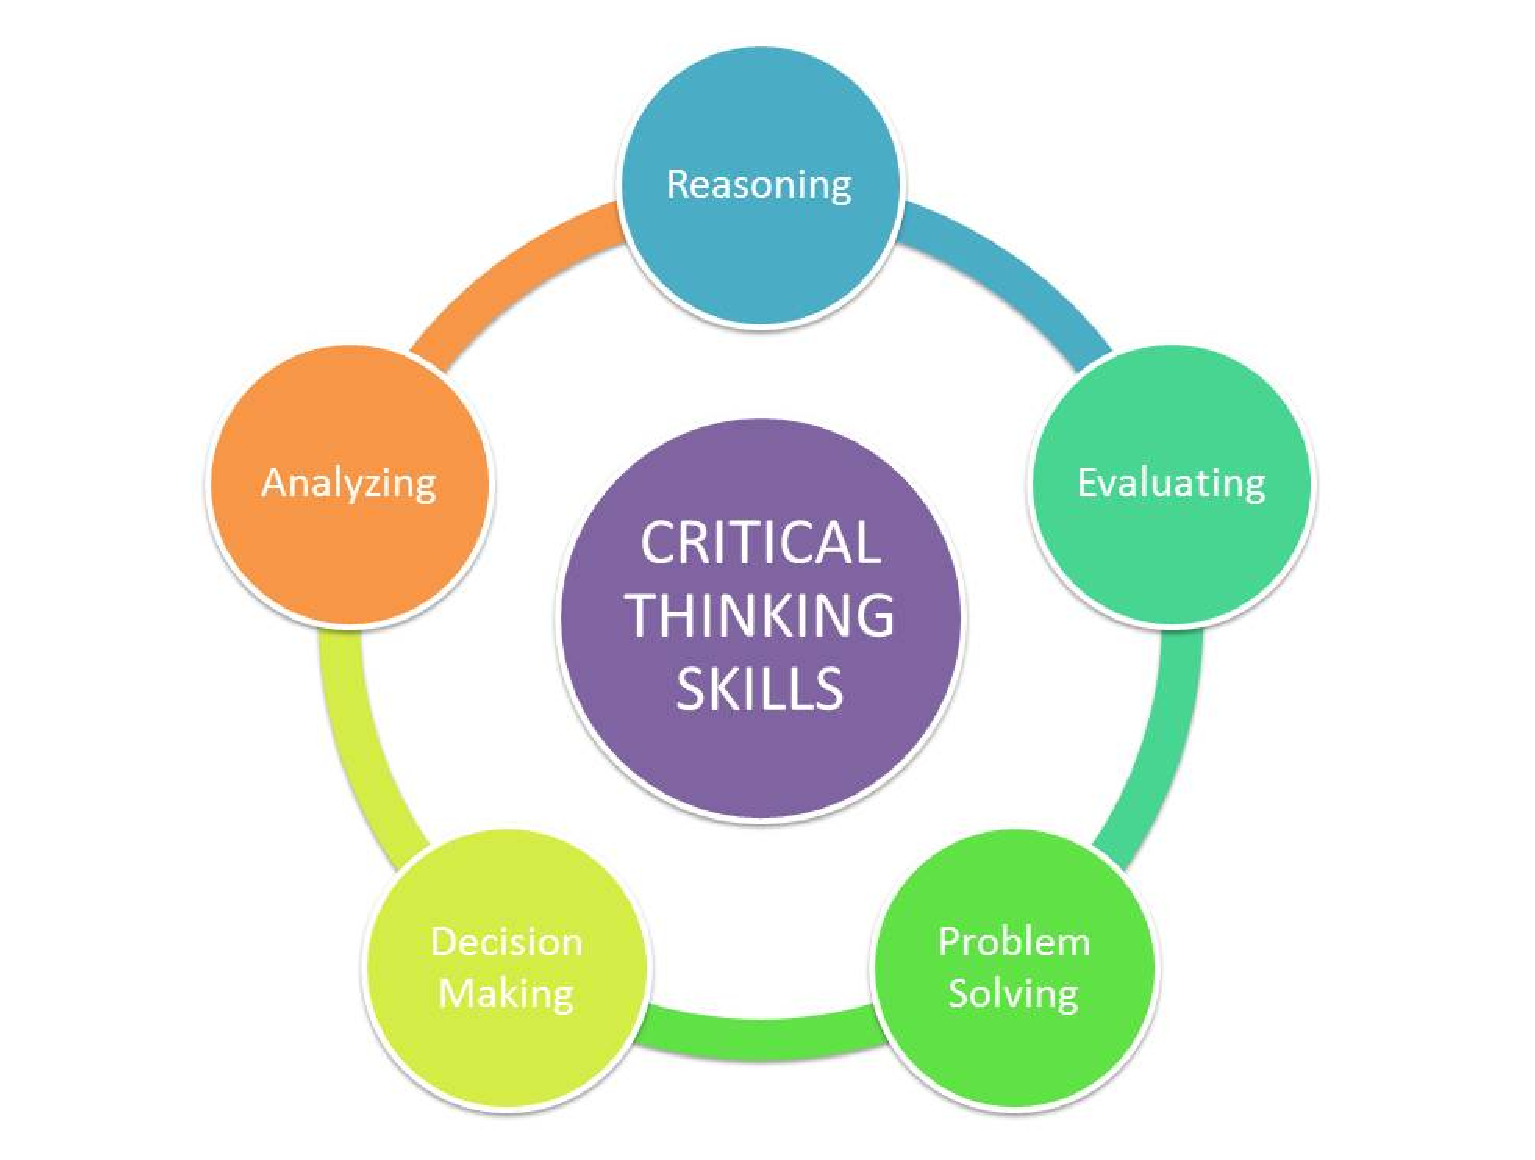
\includegraphics[width=3.5in]{figures/management/Critical_Thinking.eps}\\
  \caption{Critical_Thinking}
\end{figure}

\end{slide}
%%
%%==========================================================================================

%%==========================================================================================
%%
\begin{slide}[toc=,bm=]{Critical Thinking}

\begin{itemize}
  \item Method and application comparison table
\end{itemize}


\begin{tabular}{|c|c|c|c|c|c|c|c|}
\hline
\multicolumn{4}{|c|}{Application characteristics table} & \multicolumn{4}{|c|}{Method property table} \\
\hline
        & App 1   & App 2   & App 3 &             & Method 1  & Method 2  & Method 3\\
\hline
Charac A& $\times$  &  $\circ$  &  $\times$ & Charac A  &   $\circ$ & $\circ$   & $\times$  \\
\hline
Charac B&  $\circ$  &  $\times$ & $\circ$   & Charac B  &   $\bigtriangleup$ & $\times$  & $\circ$  \\
\hline
Charac C&  $\times$ & $\bigtriangleup$  & $\circ$   & Charac C  &   $\circ$ & $\circ$    & $\bigtriangleup$  \\
\hline
Charac D& $\bigtriangleup$ & $\times$  & $\times$   & Charac D  &  $\circ$  & $\times$   & $\times$  \\
\hline
Charac E& $\circ$  &  $\circ$  & $\circ$    & Charac E  &  $\times$ &  $\circ$   &  $\circ$   \\
\hline
Charac F&  $\times$ & $\times$ & $\times$    & Charac F  &    $\circ$  & $\bigtriangleup$  &  $\times$  \\
\hline
\hline
\end{tabular}

\vspace{0.5cm}
In Application characteristics table:

\textcolor{orange}{$\circ$}: very important,
\textcolor{orange}{$\bigtriangleup$}: not very important,
\textcolor{orange}{$\times$}: not important \\

\vspace{0.5cm}
In Method property table:

\textcolor{orange}{$\circ$}: important,
\textcolor{orange}{$\bigtriangleup$}: general,
\textcolor{orange}{$\times$}: bad

\end{slide}
%%
%%==========================================================================================

%%==========================================================================================
%%
\begin{slide}[toc=,bm=]{Critical Thinking}

\begin{itemize}
  \item According to the method and application comparison table, select the appropriate method to determine the key to innovation and method.
  \item In-depth understanding of the operating principle and mechanism of read-only and methods
  \item Organic transplantation to establish a complete ground floor ecology to support side effects.
\end{itemize}

\end{slide}
%%
%%==========================================================================================

%%==========================================================================================
%
\begin{slide}[toc=,bm=]{Questions?}
\begin{center}
\begin{figure}
    \animategraphics[autoplay, loop, height=1\textheight]{5}{figures/management//gif//question//q_}{1}{30}
\end{figure}
\end{center}
\end{slide}
%%
%%==========================================================================================

%%==========================================================================================
% TODO: Contact Page
\begin{wideslide}[toc=,bm=]{Contact Information}
\centering
\vspace{\stretch{1}}
\twocolumn[
lcolwidth=0.35\linewidth,
rcolwidth=0.65\linewidth
]
{
% \centerline{\includegraphics[scale=.2]{tulip-logo.eps}}
}
{
\vspace{\stretch{1}}
Meng Ren\\
School of Computer Science and Technology\\
Xi'an Shiyou University, China
\begin{description}
 \item[\textcolor{orange}{\faEnvelope}] \href{mailto:mren@tulip.academy}
 {\textsc{\footnotesize{mren@tulip.academy}}}

\end{description}
}
\vspace{\stretch{1}}
\end{wideslide}

\end{document}

\endinput
